\chapter{Bayesian model averaging robustness check}
\label{app:three}

\begin{figure}[!htbp]
\begin{center}
\caption{BMA - uniform g-prior and uniform model prior}
\label{fig:BMA2}
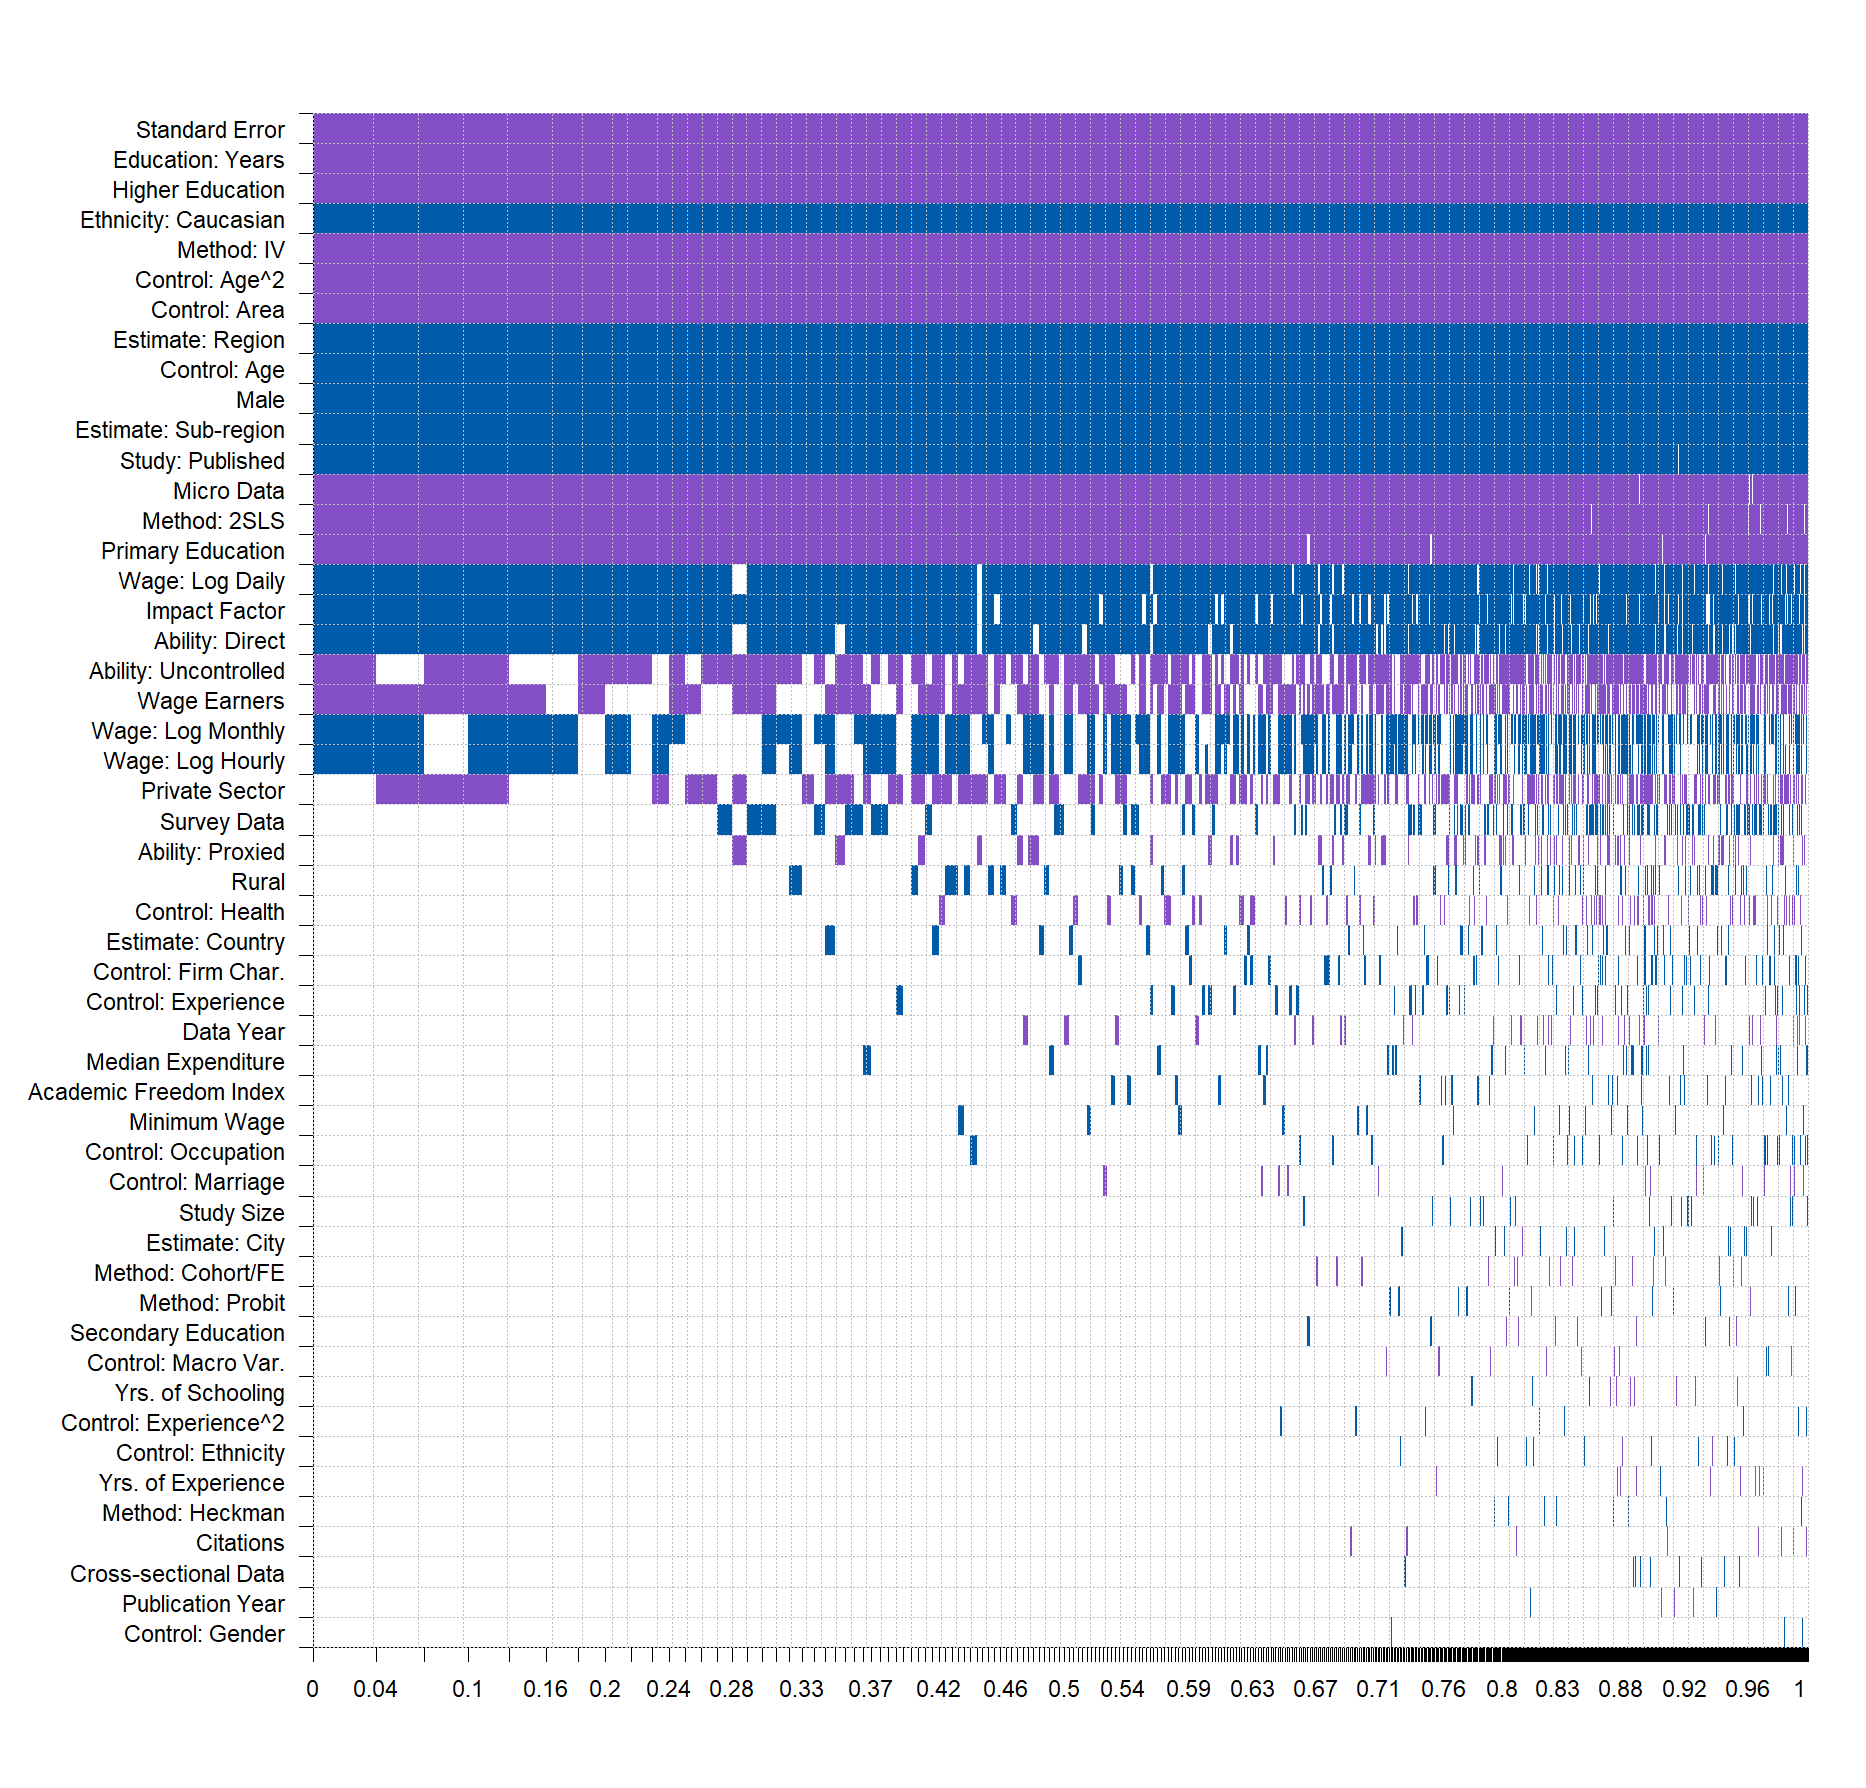
\includegraphics[width=0.8\textwidth]{Figures/BMA/bma_UIP_uniform_results.png}
\end{center}\vspace{-0.5cm}
\captionsetup{width=0.8\textwidth, font = scriptsize}
\caption*{\emph{Note:} This figure unveils the results of running the Bayesian model averaging using different specifications, namely the uniform g-prior and the uniform model prior. BMA = Bayesian model averaging. For further explanation of the procedure and individual variables, see \autoref{fig:BMA} and \autoref{tab:var}.
}
\end{figure}


\begin{figure}[!htbp]
\begin{center}
\caption{BMA - benchmark g-prior and random model prior}
\label{fig:BMA3}
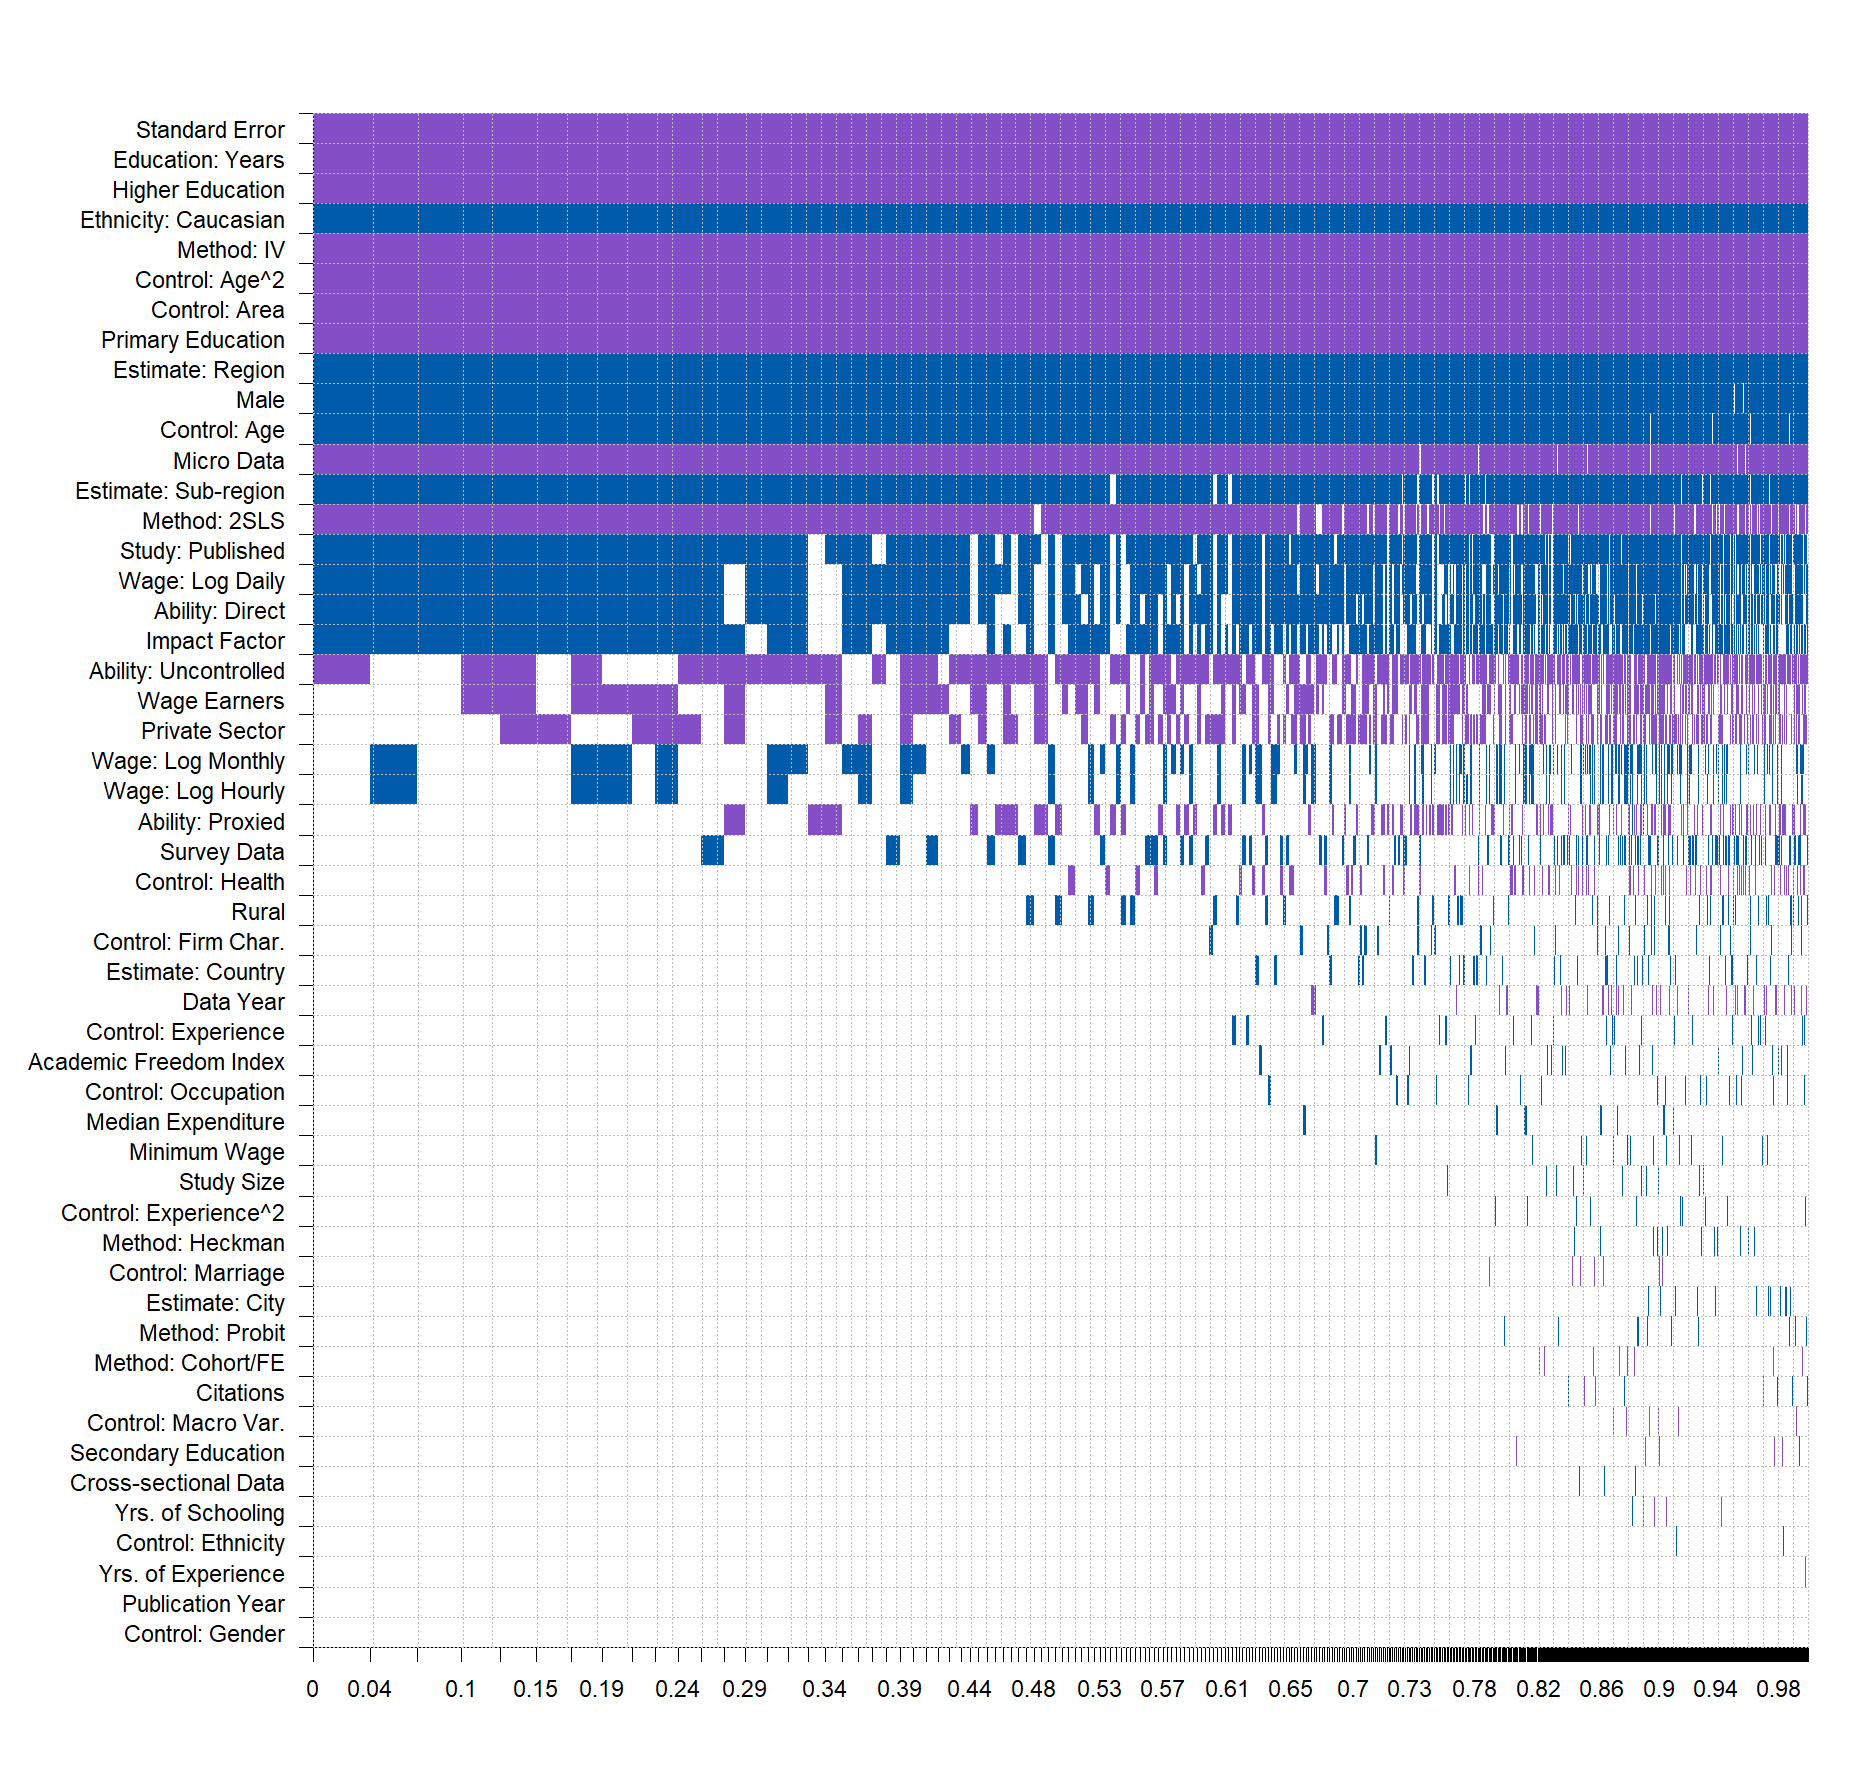
\includegraphics[width=0.9\textwidth]{Figures/BMA/bma_BRIC_random_results.png}
\end{center}\vspace{-0.5cm}
\captionsetup{width=0.9\textwidth, font = scriptsize}
\caption*{\emph{Note:} This figure unveils the results of running the Bayesian model averaging using different specifications, namely the benchmark g-prior and the uniform model prior. BMA = Bayesian model averaging. For further explanation of the method and the employed variables, see \autoref{fig:BMA} and \autoref{tab:var}.
}
\end{figure}

\begin{figure}[!htbp]
\begin{center}
\caption{BMA - HQ g-prior and random model prior}
\label{fig:BMA4}
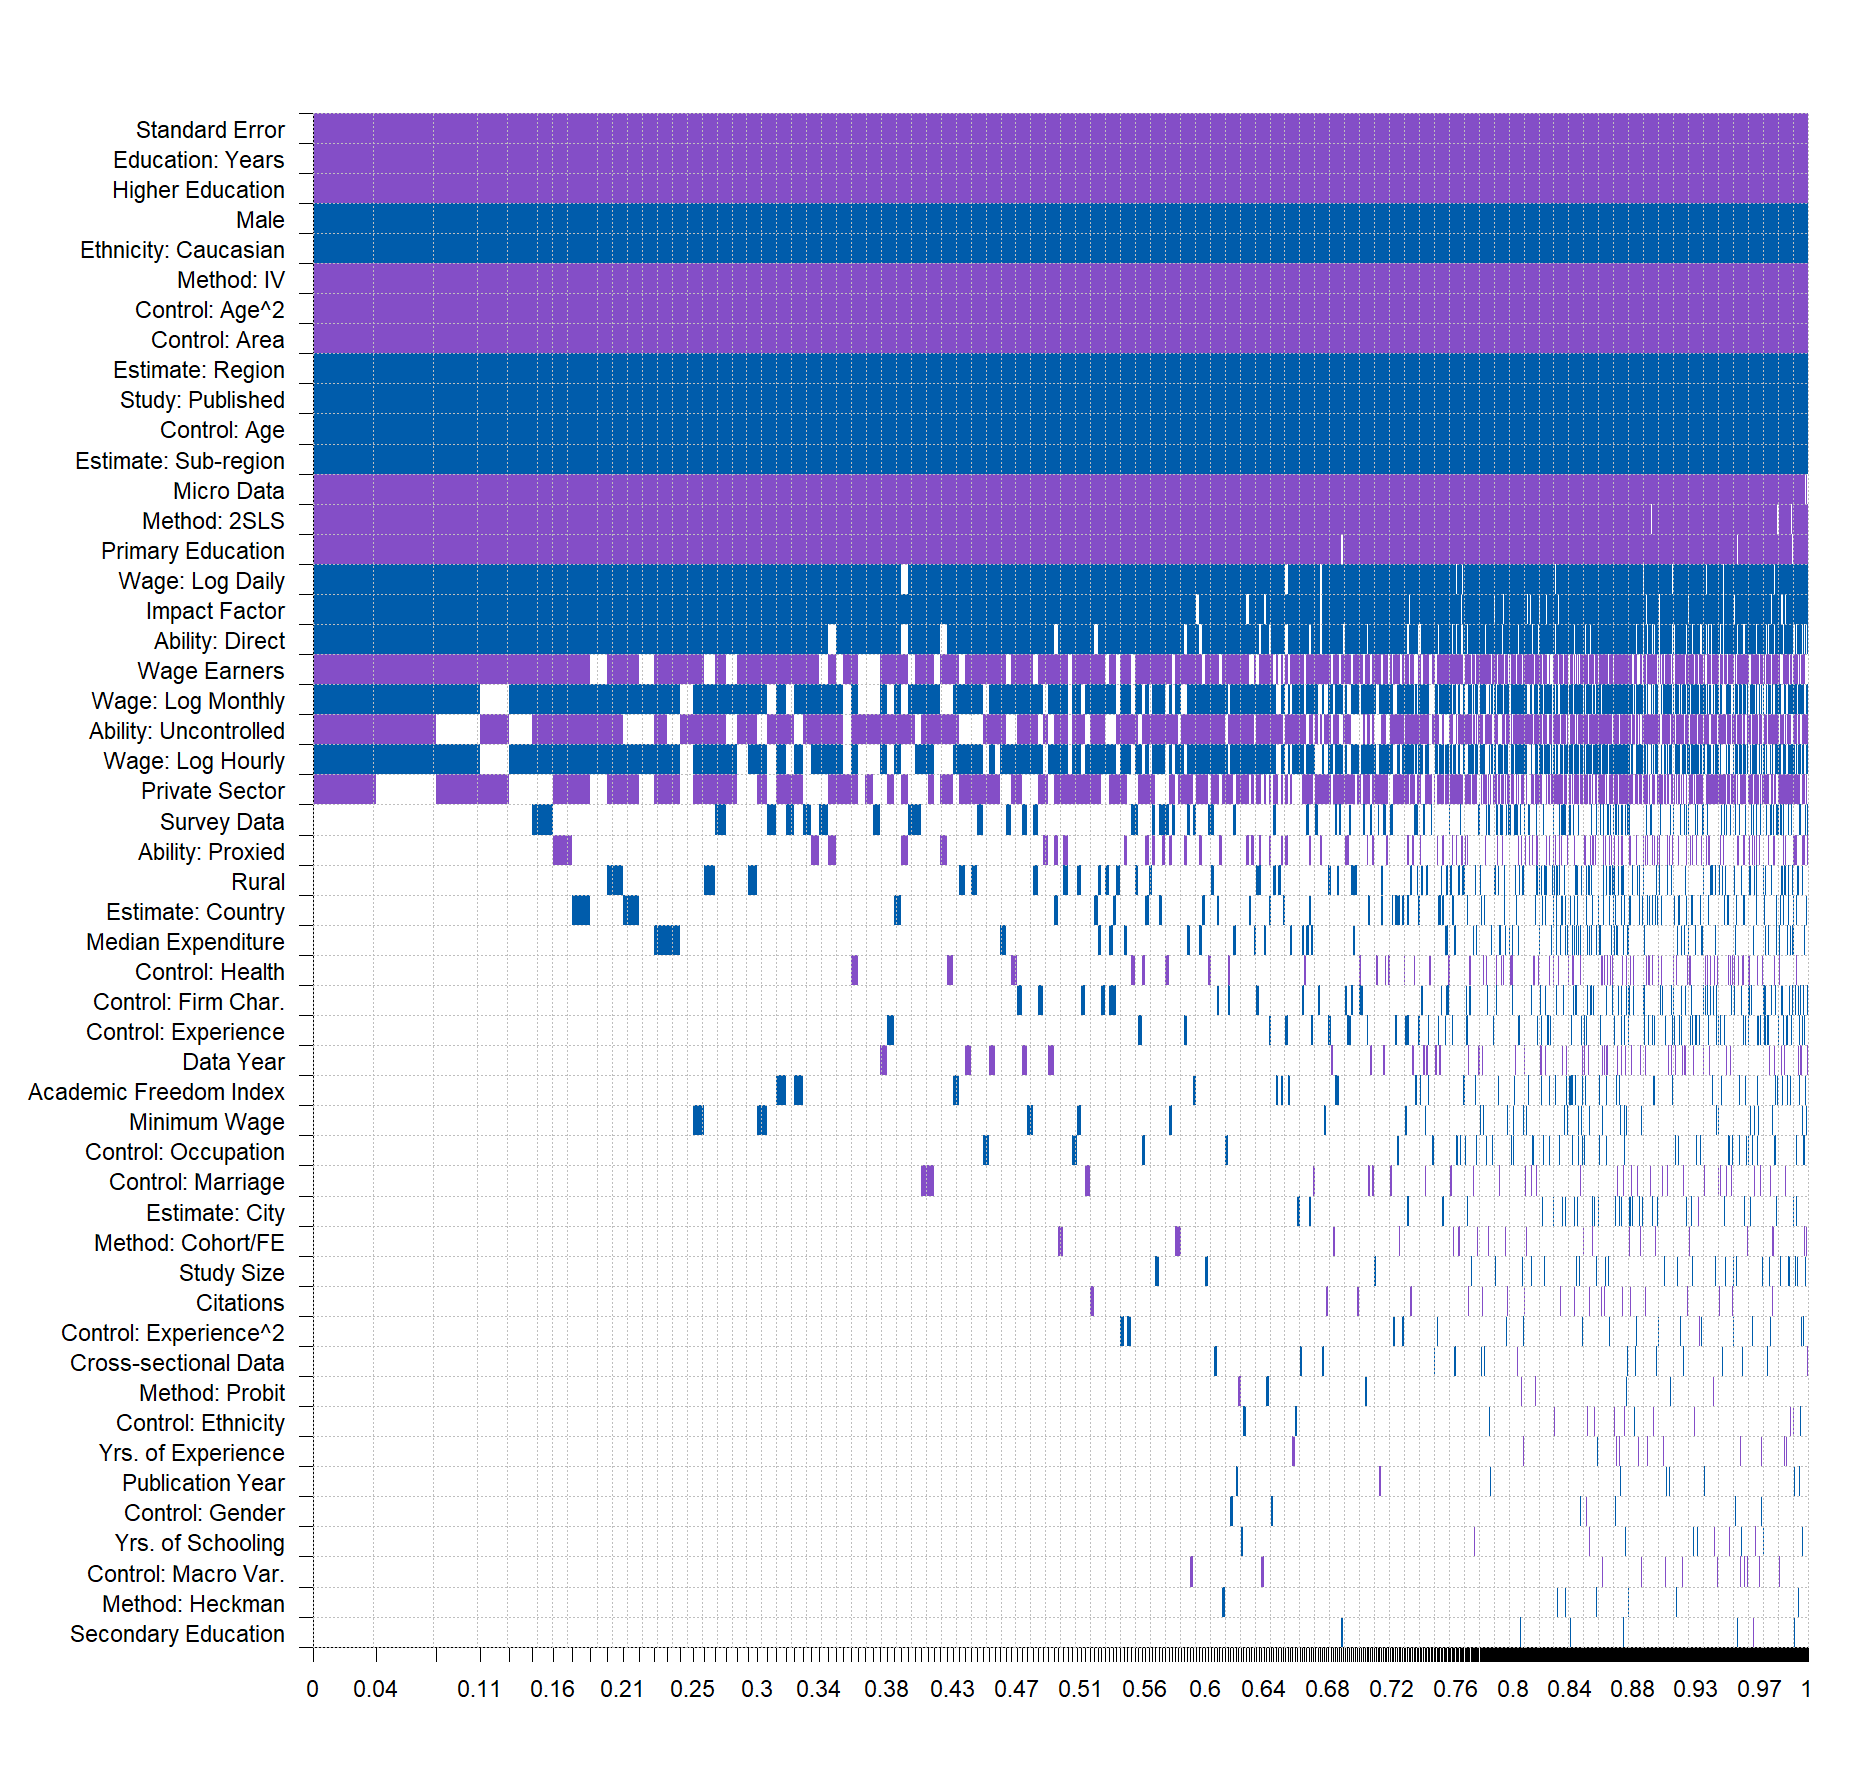
\includegraphics[width=0.9\textwidth]{Figures/BMA/bma_Hannan-Quinn_random_results.png}
\end{center}\vspace{-0.5cm}
\captionsetup{width=0.9\textwidth, font = scriptsize}
\caption*{\emph{Note:} This figure unveils the results of running the Bayesian model averaging using different specifications, namely the Hannan-Quinn criterion g-prior and the uniform model prior. BMA = Bayesian model averaging. HQ = Hannan-Quinn Criterion. For further explanation of the method and the employed variables, see \autoref{fig:BMA} and \autoref{tab:var}.
}
\end{figure}



\begin{figure}[!htbp]
\begin{center}
\caption{Bayesian Model Averaging - Correlation Table}
\label{fig:bma_corr}
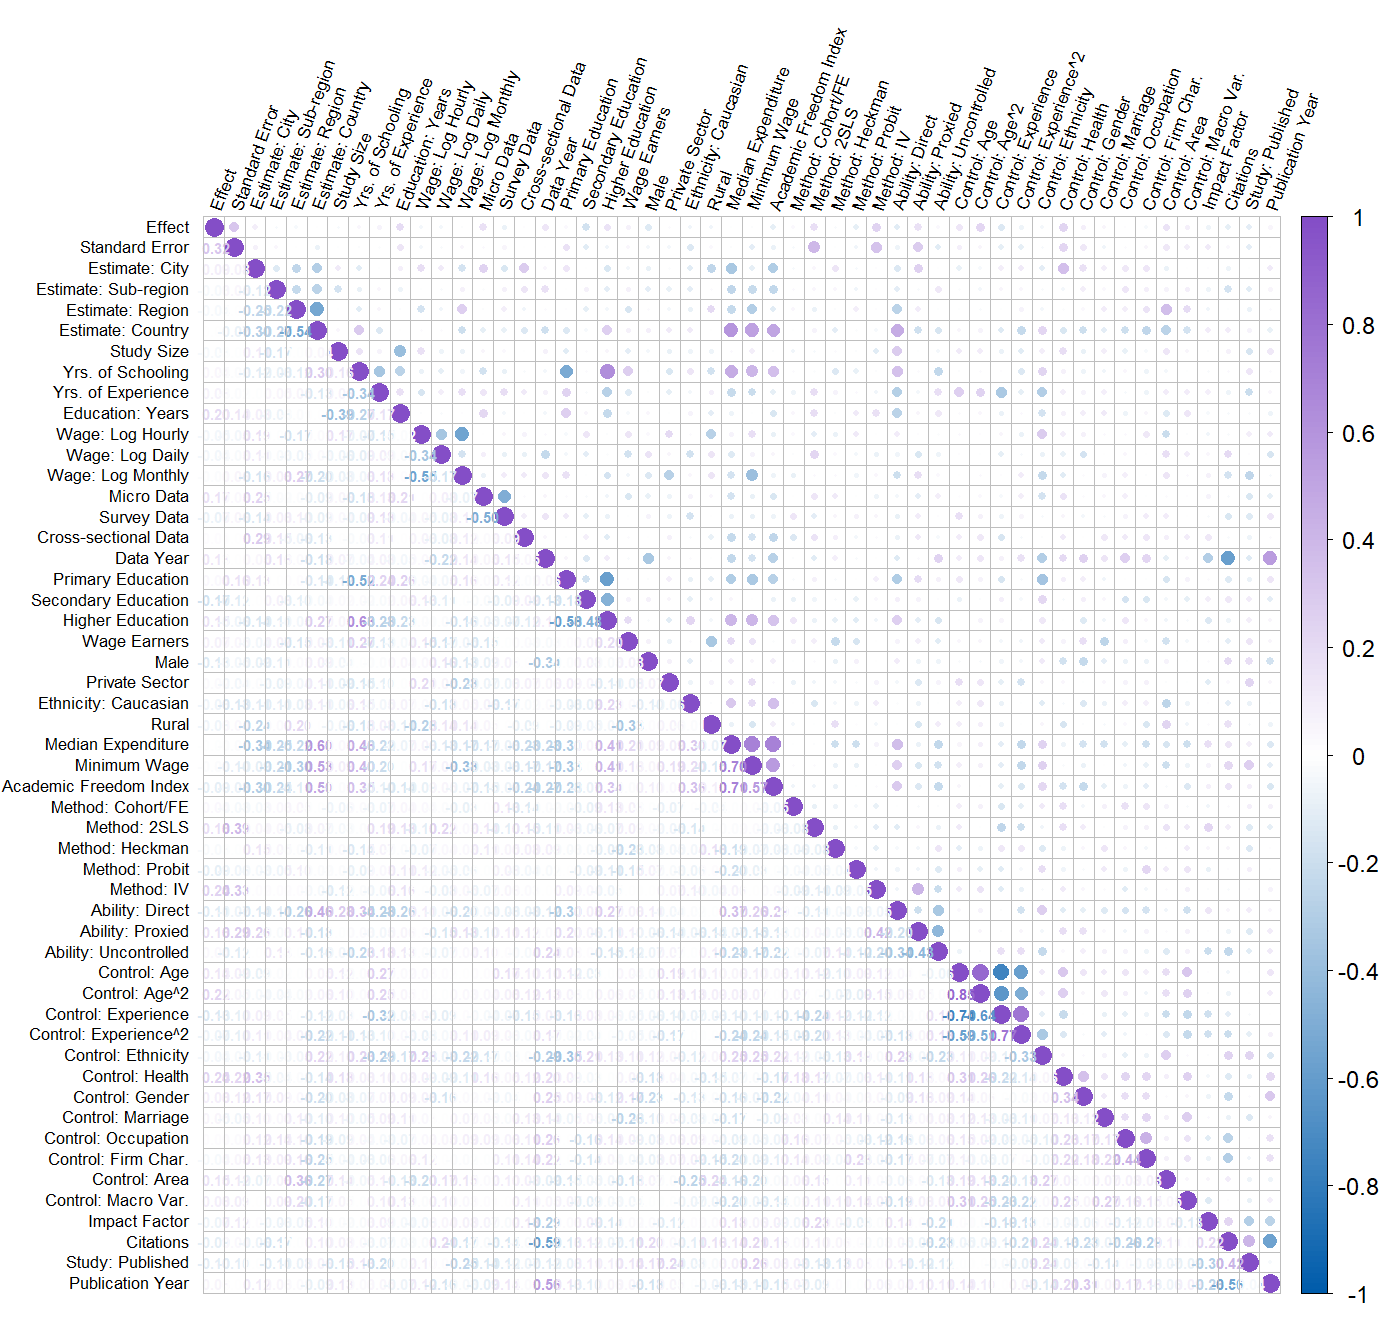
\includegraphics[width=1\textwidth]{Figures/BMA/bma_UIP_dilut_corrplot.png}
\end{center}\vspace{-0.5cm}
\captionsetup{width=0.9\textwidth, font = scriptsize}
\caption*{\emph{Note:} The figure shows the correlation between variables employed in the Bayesian model averaging. These variables are depicted on both axes. Purple color indicates a positive correlation; blue color indicates a negative correlation. Uniform g-prior and dilution model prior are used in the analysis. For results of the actual estimation, see \autoref{chap:five}. For a detailed explanation of the variables used, see \autoref{tab:var}.
}
\end{figure}



